\subsection{Introduction}
\label{ssec:intro}

Complex systems must be {\em monitored} to proactively find problems,
record/archive system health, oversee system operation, detect
malicious processes or security violations, and perform a myriad of other tasks.
The {\em monitoring subsystems} 
that perform these tasks take a wide range of forms, 
from embedded sensors that monitor physical processes to
intrusion detection systems that monitor flows to a single
organization  
to large-scale systems
that monitor the health and performance of hundreds to thousands of nodes
on the Grid.

At the heart of such monitoring systems is a complex, multifaceted
data processing problem that involves, at a minimum, the following components.
\begin{enumerate}
\item collection and aggregation of information 
distributed across the monitored system.
\item data archiving for later querying, measurement, security auditing and 
post-mortem defect detection
\item querying and information extraction from archived or current, online data
\item presentation and graphical display to administrators and users.
\end{enumerate}

A substantial part of the difficulty of building secure, reliable, efficient,
and evolving monitoring systems is the diversity, quality, and volume of data
these systems must often handle.  Often, new monitoring
systems face the problem of having to interact with legacy devices,
legacy software and legacy data, leaving implementers in a situation
where they cannot use robust off-the-shelf data management tools built for
standard formats like XML.  As a result, implementers simply
hack ``one-off'' monitoring tools of their own, which are invariably
less reliable, unoptimized, insecure, and difficult or impossible to evolve
when new requirements become known.

We call the nonstandard data formats that monitoring systems must
collect, aggregate, parse, print, archive, query, and present to 
users {\em ad hoc data formats}.   These formats, by definition,
have no standard data processing tools associated with them.
\figref{figure:data-sources} presents a selection of such formats
used in a variety of different monitoring systems.
They include ASCII, binary, and Cobol data formats, with
both fixed and variable-width records, ranging in size from
relatively small files through network applications which process over
a gigabyte per second.  Common errors in the data include undocumented data,
corrupted data, missing data, and multiple missing-value
representations.

\begin{figure*}
\begin{center}
\begin{tabular}{|l|l|l|l|l|}
\hline
Name \& Use   &  Representation              &Size           & Common Errors \\ \hline\hline
Web server logs (CLF): &  Fixed-column  & $\leq$12GB/week & Race conditions \\ 
Measuring web workloads         &  ASCII records &                 & on log entry \\
                                &                &                 & Unexpected values\\ \hline
CoMon data:              &  Geographically & 600 MB/day & Race conditions on\\ 
Monitor \& troubleshoot  &  distributed    & collected from           & log entry \\
PlanetLab infrastructure &  ASCII records  & \appr{}400-450 machines           & \\\hline
AT\&T provisioning data (\dibbler{}): & Variable-width  & 2.2GB/week & Unexpected values \\ 
Monitoring service activation & ASCII records  &            & Corrupted data feeds \\ \hline
Phone call detail:   &  Fixed-width   &\appr{}7GB/day &  Undocumented data\\ 
Fraud detection & binary records & & \\  \hline 
AT\&T billing data (\ningaui{}): & Various Cobol  & \appr{}4000 files/day, & Unexpected values\\ 
Monitoring billing process   & data formats            & 250-300GB/day    & Corrupted data feeds \\ \hline
IP backbone data (\darkstar{})  & ASCII  & $\ge$ 15 sources  & Multiple missing-value \\
Monitoring network performance  &        & \appr{}15 GB/day              & representations  \\ 
                                &        &                               & Undocumented data \\\hline
Netflow       & Data-dependent \# of     & $\ge$1Gigabit/second  & Missed packets\\ 
Monitoring network performance              &  fixed-width    &                       & \\ 
               & binary records & & \\ \hline
\end{tabular}
\caption{Selected ad hoc data sources for system monitoring. }
\label{figure:data-sources}
\end{center}
\end{figure*}

Processing this sort of 
ad hoc data is challenging for a variety of other reasons. 
First, when the data comes from legacy software, sources or devices, it 
typically just arrives ``as is'': the analysts
who receive it can only say ``thank you,'' not request a more
convenient format.  Second, documentation for the format may not exist
at all, or it may be out of date.  A common phenomenon is for a field
in a data source to fall into disuse.  After a while, a new piece of
information becomes interesting, but compatibility issues prevent data
suppliers from modifying the shape of their data, so instead they
hijack the unused field, often failing to update the documentation in
the process.

Third, such data frequently contain errors, for a variety of reasons:
malfunctioning equipment, race conditions on log entry~\cite{wpp},
non-standard values to indicate ``no data available,'' human error in
entering data, unexpected data values, \etc{} The appropriate response
to such errors depends on the application.  Some applications require
the data to be error free: if an error is detected, processing needs
to stop immediately and a human must be alerted.  Other applications
can repair the data, while still others can simply discard erroneous
or unexpected values.  For some applications, errors in the data can
be the most interesting part because they can signal where two systems
are failing to communicate.  Monitoring systems may need to respond to such
errors immediately and effectively.

Fourth, online monitoring systems
are highly susceptible to attack from malicious outsiders.
For example, intrusion detection systems
and performance evaluation systems that monitor network activity 
may be sent malicious packets or other data that cause buffer overflows
and allow attackers to take control of, evade, dismantle or corrupt these
systems.  A cautionary example of the dangers of online ad hoc data
processors is the Ethereal system~\cite{ethereal}. Ethereal is used by network administrators for monitoring, analyzing
and troubleshooting networks. Unfortunately, like most network software, users have found a number of
vulnerabilities in the software, and moreover many of these vulnerabilities are directly related to the mundane
components of the system that parse ad hoc data as opposed to the parts of the system that perform
higher-level tasks. For instance, in March 2004, Stefan Esser posted an advisory on 13 different buffer over-
flow attacks on Ethereal~\cite{etherealvulnerabilities}. Of the 13, 9 attacks occurred during parsing. These problems are not merely theoretical -- it was
a buffer overflow in a security monitoring system that was exploited by the
Witty Worm~\cite{witty}.

Fifth, ad hoc data sources can be high volume:
AT\&T's call-detail stream contains roughly 300~million calls per day
requiring approximately 7GBs of storage space. Although this data is
eventually archived in a database, analysts mine it profitably before
such archiving~\cite{kdd98,kdd99}. More challenging, the \ningaui{}
project at AT\&T accumulates billing data at a rate of 250-300GB/day,
with occasional spurts of 750GBs/day. Netflow data arrives from Cisco
routers at rates over a gigabyte per second~\cite{gigascope}! Such
volumes mean performance is critical and it certainly
must be possible to process the data without loading
it all into memory at once.

Finally, before anything can be done with an ad hoc data source,
someone has to produce a suitable parser for it.  Today, people tend
to use \C{} or \perl{} for this task.  Unfortunately, writing parsers
this way is tedious and error-prone, complicated by the lack of
documentation, convoluted encodings designed to save space, the need
to produce efficient code, and the need to handle errors robustly to
avoid corrupting downstream data.  Moreover, the parser writers'
hard-won understanding of the data ends up embedded in parsing code,
making long-term maintenance difficult for the original writers and
sharing the knowledge with others nearly impossible.

\paragraph*{Data-centric Monitor Generation}
We propose {\em data-centric monitor generation}, a new paradigm
for construction system monitors, in which programmers
specify the shape and properties of data manipulated by
the monitoring system and a compiler automatically
generates efficient, reliable, and secure
monitoring tools from that specification.
More specifically, the system will consist of the 
following components:

\begin{enumerate}

\item A high-level specification language to describe a monitor's
data sources.  The specification language will be able to
concisely and accurately describing any ad hoc data source,
including its format, semantic properties, location, and
temporal attributes in an easy-to-understand, easy-to-modify syntax.

\item A compiler that takes data specifications as inputs and
automatically generates a suite of 
efficient data processing libraries for parsing, printing, error detection
and correction, distributed data gathering, compression, and 
reformatting of ad hoc data.

\item A fully automatic tool generator that links the compiler-generated 
libraries to format-independent tool stubs to produce easy-to-use 
tools for high-level tasks including data display and querying.

\end{enumerate}

\begin{figure}[t]
\begin{center}
\centerline{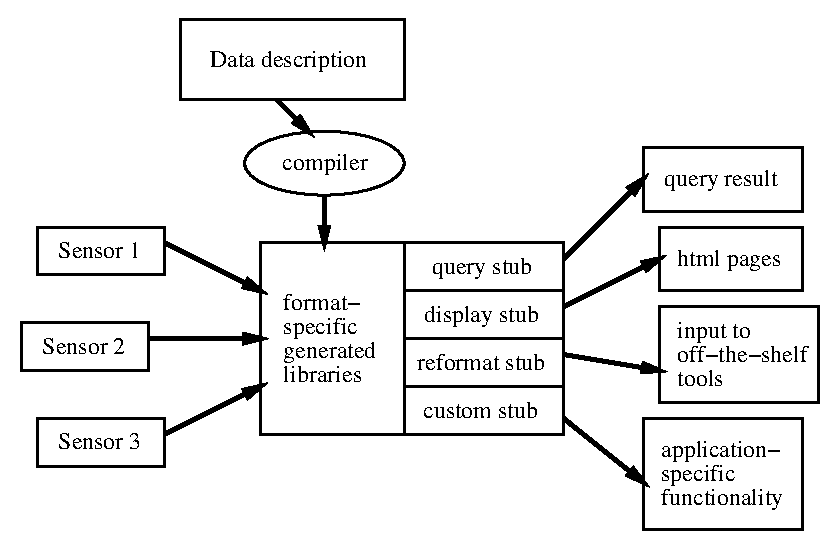
\psfig{file=arch_idraw_edit.ps,height=2.5in}}
\end{center}
\caption{\label{fig:arch} Architecture of Data-centric Monitor Generator.
}
\end{figure}

In the follow section, we will explain 
the architecture of a data-centric monitor generation system
and our prototype language design in more detail.  
Next, we will explain more of the specifics concerning
the generated tool suite for system monitoring.
In Section~\ref{ssec:features}, we will highlight some of the most
important language design challenges we face and
in Section~\ref{ssec:semantics}, we will propose a
formal system analysis to identify implementation errors
and improve system reliability.
In Section~\ref{ssec:impact}, we will explain how our research
on automatic generation of data processing tools
will make a broad impact on data processing that must be done
in disciplines well outside the bounds of
traditional computer science ranging from microbiology to physics to
economics.  We will also explain our education plan.
